% IEEE conference template (IEEEtran). Compile with XeLaTeX for the Arabic text:
%   latexmk -xelatex main.tex      (or: xelatex, bibtex, xelatex, xelatex)
\documentclass[conference]{IEEEtran}
\usepackage{fontspec}
\setmainfont{Times New Roman}
\usepackage{cite}
\usepackage{amsmath,amssymb,amsfonts}
\usepackage{graphicx}
\usepackage{textcomp}
\usepackage{xcolor}
\usepackage{booktabs}
\usepackage{threeparttable}
\usepackage{array}
\usepackage{url}
% Arabic: XeTeX's own right-to-left support (TeX--XeT) instead of polyglossia/bidi, which would
% override IEEEtran's caption style.
\TeXXeTstate=1
\newfontfamily\arabicfont[Script=Arabic,Scale=1.15]{Sakkal Majalla}

\usepackage[hidelinks]{hyperref}

\newcommand{\todo}[1]{\textcolor{red}{[#1]}}
\newcommand{\ar}[1]{{\arabicfont\beginR #1\endR}}

\begin{document}
\bstctlcite{IEEEexample:BSTcontrol}

\title{Is Generative AI Displacing Arabic? Perceived Change in Arabic Use Among Arabic--English Bilinguals in Lebanon}

\author{\IEEEauthorblockN{Hadi Ghazi}
\IEEEauthorblockA{\textit{Lebanese University}\\
hadigghazi@gmail.com}}

\maketitle
\thispagestyle{plain}
\pagestyle{plain}

\begin{abstract}
Generative AI works better in English than in Arabic, so bilinguals who rely on it may route more of their work through English. In an anonymous Arabic online survey of 40 bilingual AI users (primary sample: 37 who grew up in the Arab region and live in Lebanon), respondents rated whether, because of AI, they now use Arabic less or more in eight domains. Most reported AI-attributed decreases in work or study (25 of 36, none reporting more) and in writing messages, and decreases outnumbered increases for formal Arabic (16 against 3). The decreases followed the order predicted by domain theory, from work and study to personal matters to family, an order that may also reflect where AI is used. The predicted larger decrease for formal than for dialect domains was not found. How intensively people use AI, the language they use with it and the quality gap they perceive did not jointly predict the reported decrease. In cross-validated machine learning, AI-use information added no detectable predictive value, and no model was usable. Oversampling inside the training folds did not help, and oversampling before the train--test split produced spurious models with an apparent area under the curve of up to 0.96. The AI attribution went together with blaming social media. Respondents attribute a decrease in their Arabic to AI, but the data cannot show that AI causes it or separate this attribution from a broader sense that technology is eroding Arabic.
\end{abstract}

\begin{IEEEkeywords}
generative AI, Arabic, language shift, diglossia, perceived language change, survey, machine learning
\end{IEEEkeywords}

% =====================================================================================================
\section{Introduction}

Generative AI tools perform less well in Arabic than in English. Tool-calling accuracy drops when the same tasks are prompted in Arabic \cite{kubrak2025}, and four chatbots answered the same infectious-disease questions less well in Arabic than in English \cite{sallam2024}. Bilinguals who use these tools daily may therefore do more of their AI-assisted tasks in English. Arabic was losing formal domains to English before generative AI. English dominates higher education in the UAE \cite{albataineh2021}, where students at English-medium universities report weaker academic Arabic \cite{masri2019}; Qatar University students rate English more useful than Arabic for scientific and professional communication \cite{mustafawi2022}; and in Lebanon, a small interview study found English used across education and professional life \cite{mehio2026}.

Research on generative AI and its users' language skills has looked almost entirely at second-language learning, e.g., \cite{saarela2026}. The closest work on Arabic records which language Tunisian users choose with ChatGPT \cite{bouzayenne2026} but does not ask whether that choice affects their Arabic elsewhere. To our knowledge, no study has asked Arabic speakers whether they attribute changes in their own Arabic use to AI.

This study asks Arabic--English bilinguals in Lebanon in which domains, and in which direction, they report that AI has changed their use of Arabic (RQ1); whether AI-use intensity, the English share of AI use and the perceived Arabic--English quality gap predict that change (RQ2); whether the change goes with perceived difficulty using Arabic without AI and mediates the link from AI use (RQ3); and whether AI-use information improves out-of-sample prediction of who reports AI-attributed decreases beyond background characteristics (RQ4). The outcome is the change that respondents attribute to AI. It is not a measure of language loss, and it is compared with a rival attribution to social media (one item).

% =====================================================================================================
\section{Background and Hypotheses}

\emph{Domains and diglossia.} Language use is organised by domains such as family, friendship, religion, education and work, and a dominant language displaces a weaker one domain by domain, starting with public and formal domains \cite{fishman1965,fishman1972}. Arabic is diglossic: Fusha (Modern Standard Arabic) carries the formal, written functions and the spoken dialect the everyday ones \cite{ferguson1959}, so formal functions should be lost first. Hence \textbf{H1}: net AI-attributed change is negative for Fusha (H1a) and for work or study (H1b); and \textbf{H2}: the decrease follows the order work/study $>$ personal matters $>$ family (H2a) and is larger for Fusha than for the dialect domains of self-talk, personal matters, and family and friends (H2b).

\emph{Why AI could matter.} Adult first-language attrition is usually explained by reduced use of the first language and interference from an active second language \cite{chaouch2025,gallo2025}. It has been studied mainly in migrants; in the home country the first language holds up better. Students at English-medium universities in Turkey showed no deficit on Turkish tests, although their self-rated Turkish writing fell more often than that of Turkish-medium peers \cite{aycicegi2015}. Generative AI could add a new route to reduced use. Once access to a technology is equal, inequality moves from access to what people can do with it \cite{hargittai2002}, and AI lets people do more in English. Hence \textbf{H3}: AI-use intensity (H3a), the share of AI use in English (H3b) and the perceived quality gap (H3c) predict the AI-attributed decrease; \textbf{H4}: the decrease is associated with perceived difficulty using Arabic without AI; and \textbf{H5}: the decrease mediates the link from AI-use intensity to that difficulty.

\emph{Measuring attributed change.} Wirtz and Pickl \cite{wirtz2025} showed that people can rate in an online survey how a major life event changed their language use, on a scale with a true zero (``no change''). Such retrospective attributions are only partly accurate. Perceived change after life events matched measured personality change only modestly and also tracked trends that began before the event \cite{schwaba2023}. This study adapts the format to AI and reads the results as attributions.

% =====================================================================================================
\section{Method}

\subsection{Design, Procedure and Participants}

An anonymous Google Form in Arabic (seven pages; 25 closed questions, five grids and one optional open question) was open from 30 September 2026, 17:57, to 1 October 2026, 22:15; 36 of the 40 responses arrived on the first day. Respondents were recruited through university WhatsApp groups, friends and LinkedIn. Collection was closed at 40 responses, against a planned 150 collected and about 120 analysed, before any analysis. The scheduled back-translation and pretest did not take place, and only the author reviewed the wording before launch. The Arabic wording is therefore the instrument (Appendix), and the English used here is the author's source wording. The advertised duration of about seven minutes was not timed. The first page described the survey as a research project at the Lebanese University, voluntary and anonymous (no names or contact details, so a response could not be withdrawn after submission) and reported only as group results; respondents confirmed being 18 or older and agreeing to take part. A screening question required Arabic as first language, use of English for study or work, and weekly AI use for six months or more.

All 40 respondents consented and passed the screening question; one, who began regular AI use in 2026, may not meet the six-month criterion (the start month was not asked). Following the analysis plan, the primary sample holds migration constant. It comprises the 37 respondents who grew up and live in the Arab region and have not moved country since 2022; one who grew up and lives outside the Arab world and two who moved were excluded. Of the 37, 35 grew up in Lebanon and 2 in the Gulf, and all live in Lebanon. Thirty-two were under 25 and five were 25--34, 20 were women, 22 were studying for or held a master's degree or higher and 14 a bachelor's degree, and 26 studied or worked in computing. Thirty used AI several times a day and 19 always wrote to it in English. All 40 are analysed as a sensitivity check.

\subsection{Measures}

The core grid asked: \emph{``Because of AI, do you now do each of these less or more?''} (\ar{بسبب الذكاء الاصطناعي، هل أصبحت تقوم بكلٍّ مما يلي أقل أم أكثر؟}), comparing now with before regular AI use, from \emph{much less} ($-2$) through \emph{no change} (0) to \emph{much more} ($+2$). The eight domains are shown in Fig.~\ref{fig:profile} and, as fielded, in the Appendix. A preceding grid recorded which language each activity is mostly done in today, with a ``not applicable'' option; a domain marked not applicable was set to missing. The \emph{displacement score} is minus the mean change over the applicable domains (at least six), so higher means more AI-attributed decrease ($\alpha=0.88$; McDonald's $\omega=0.88$, bootstrap 95\% CI [0.75, 0.93] \cite{dunn2014}; $n=30$ complete cases). Because this consistency may partly reflect a general tendency to blame AI, the score is read as the decrease a person attributes to AI and is not treated as a measure of domain loss.

\emph{Perceived difficulty without AI}: ``Because of AI, has each of these become harder or easier for you, when you use Arabic on your own without AI?'' (finding the everyday word, speaking one's dialect fluently, saying what one means fully in Arabic; higher = harder; $\alpha=0.78$, $\omega=0.83$ [0.62, 0.93]; 24 of 37 scored exactly 0). \emph{AI use}: frequency, share of work or study done with AI, breadth (number of eight uses ticked), year regular use began, the language used to write to AI (English share), and exposure to AI-generated content and the language chosen for it. \emph{AI-use intensity} is the mean of the standardised share and breadth (as planned, frequency is descriptive only; 30 of 37 are in its top category). \emph{Perceived quality gap}: four agreement items, one reversed ($\alpha=0.68$, $\omega=0.69$). Also asked: a substitution item (``Has it happened that you did something in English, although you could have done it in Arabic, because AI helps you better in English?''), the same change question for social media over the same period (one item, after the AI grid), life events during the period, expected change in each domain in two years, and English level.

Three safeguards in the analysis plan were not fielded: a reminder to choose ``no change'' if a change had other causes (such as university or a new job), a placebo row, and an attention check. The practice items and five planned items were also dropped before launch, so the checks that relied on them could not be run.

\subsection{Analysis}

The analysis follows a plan written before data collection (27 September 2026; not registered) and a study proposal (30 September). Five decisions taken after the data were seen are reported with their alternatives: returning to the plan's core sample after a first pass on all 40 (with all 40, H4 is not supported); averaging all eight fielded domains instead of the plan's four; adjusting for age and an English-medium start only (adding the plan's field and AI tenure changes no conclusion); setting aside the plan's rule for samples below 100 (H5 as the only confirmatory test, age as the only covariate, a logistic baseline as the only machine learning), except that H5 is reported as underpowered; and writing the machine-learning design after data collection.

Family A (H1--H2, within-person) used Wilcoxon signed-rank tests against zero, with exact sign tests alongside for H1a and H1b, and Page's one-sided test for the predicted order \cite{page1963}, with Friedman's test and Kendall's $W$. Family B regressed the displacement score on the three AI-use measures (H3, evaluated by their joint test) and perceived difficulty on the displacement score (H4), using OLS with HC3 standard errors and $t$-based inference \cite{long2000}, adjusted for age 25 or over and starting English-medium study or work. Holm's correction \cite{holm1979} was applied within each family, and a wild bootstrap (Rademacher weights, null imposed) checked the Family B $p$-values \cite{davidson2008}. H5 followed PROCESS model 4 \cite{hayes2022} with a 5000-resample percentile bootstrap; at $n=36$ it can detect only large paths \cite{fritz2007}. A Firth logistic regression \cite{firth1993} of any net decrease checked H3 in binary form. Analyses were run in SPSS 23 \cite{spss23} and Python \cite{seabold2010,virtanen2020}; 34 statistics computed in both agree.

\subsection{Machine Learning (RQ4)}

The machine learning is exploratory. Its design was written after data collection, once the class counts and one table of feature--target correlations had been seen. A first full run was audited independently and revised before the results reported here; among other changes, a school-language feature that had been added after the correlations were seen was removed. Targets were the number of domains with a decrease (regression), any decrease in a formal domain (work or study, or Fusha) and a decrease in each single domain with at least eight respondents in the smaller class (six domains; family and religion had too few). Features came in nested blocks: background (age 25 or over, computing field, education, English level, English-medium start), then plus AI use (seven items), then plus the quality gap; outcome items were never features. Models had fixed settings (L2 logistic or ridge regression as the primary model, random forest, gradient boosting) and were evaluated by repeated 10$\times$5-fold cross-validation, with class imbalance handled by oversampling (SMOTENC \cite{chawla2002}, applied inside the training folds only). Paired comparisons used the Nadeau--Bengio corrected $t$ \cite{nadeau2003}; whether a model beat chance was tested by permutation (outcome shuffled, whole pipeline refit, 500 permutations), with Holm's correction. Three further targets named before data collection (substitution, expected decrease in two years, any perceived difficulty) were added later, with criteria for a usable model fixed before they were modelled: above chance after correction; stable over ten other random splits (mean AUC at least 0.70, none below 0.65; for a count, $Q^2>0$ throughout and a significant gain over the mean); not dependent on age; balanced accuracy at least 0.65. Models used scikit-learn and imbalanced-learn \cite{pedregosa2011,lemaitre2017}.

% =====================================================================================================
\section{Results}

\subsection{Where Respondents Report Change (RQ1)}

Thirty-one of the 37 respondents reported an AI-attributed decrease in at least one domain (3.2 of their applicable domains on average). Decreases were most common in work or study (69\% [53, 82], none reporting more) and writing messages and posts (57\%), and least common with family and friends (19\%) and for religious texts, where decreases and increases balanced (9\% each); for Fusha, 16 of the 33 to whom it applied reported less and 3 more (Fig.~\ref{fig:profile}). Two thirds (25 of 37, 68\% [51, 80]) reported at least sometimes doing in English what they could have done in Arabic, because AI works better in English.

\begin{figure}[t]
\centerline{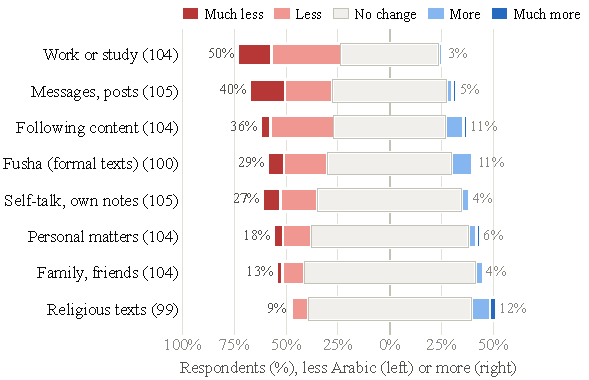
\includegraphics[width=\columnwidth]{fig1_domain_profile_column.pdf}}
\caption{AI-attributed change in Arabic use by domain (primary sample), centred on ``no change''; $n$ in parentheses excludes respondents who marked the domain not applicable.}
\label{fig:profile}
\end{figure}

\subsection{Direction and Order (H1--H2)}

The net change was negative for Fusha (H1a) and for work or study (H1b), and the decrease followed the predicted order work/study $>$ personal matters $>$ family (H2a; Table~\ref{tab:confirm}). These results held with all 40 respondents (Holm $p\leq0.026$). The plan's own test of H1b and H2a, restricted to people whose work or study setting did not change, could not be run as intended: only eight respondents met a proxy for it (work or study: 3 less, 0 more, $p=0.25$; order: $n=7$, Page one-sided $p=0.062$). The decrease for Fusha was not larger than for the dialect domains (H2b).

\begin{table*}[t]
\centering
\begin{threeparttable}
\caption{Confirmatory Tests (Primary Sample)}
\label{tab:confirm}
\footnotesize
\begin{tabular}{@{}llllll@{}}
\toprule
Hypothesis & $n$ & Result & Test & Holm $p$ & Verdict \\
\midrule
\multicolumn{6}{@{}l}{\emph{Family A: direction and order of AI-attributed change}}\\
H1a Fusha & 33 & 16 less, 3 more & $z=-3.04$, $r=-0.53$ & 0.005 & supported \\
H1b Work or study & 36 & 25 less, 0 more & $z=-4.56$, $r=-0.76$ & $<$0.001 & supported \\
H2a Work/study $>$ personal $>$ family & 34 & means 0.97, 0.41, 0.15 & Page; $\chi^2(2)=30.16$, $W=0.44$ & $<$0.001 & supported \\
H2b Fusha $>$ dialect domains & 33 & difference $+0.12$ & $z=1.14$ & 0.26 & not supported \\
\midrule
\multicolumn{6}{@{}l}{\emph{Family B: H3 predicts the displacement score; H4 predicts difficulty from it} ($n=36$, HC3)}\\
H3 (joint) & 36 & three predictors & $F(3,30)=1.46$, $p=0.24$ & & not supported \\
\quad H3a AI-use intensity & & $b=-0.01$ [$-0.21$, 0.19] & $p=0.95$ & 0.95 & \\
\quad H3b English share of AI use & & $b=0.22$ [0.005, 0.43] & $p=0.045$ & 0.14 & \\
\quad H3c Perceived quality gap & & $b=-0.12$ [$-0.40$, 0.17] & $p=0.41$ & 0.82 & \\
H4 Difficulty without AI & 36 & $b=0.44$ [0.14, 0.75] & $p=0.006$ & 0.024 & supported$^{a}$ \\
H5 Mediation & 36 & indirect $-0.02$ [$-0.14$, 0.04] & percentile bootstrap & & not supported$^{b}$ \\
\bottomrule
\end{tabular}
\begin{tablenotes}[flushleft]\footnotesize
\item Wilcoxon tests against zero (for H1a and H1b, exact sign tests agree); H2a: Page's one-sided test, complete-case means. Family B adjusts for age 25 or over and an English-medium start; brackets are 95\% CIs. $^{a}$Holm-significant in about half of the specifications, not after removing any one of three influential respondents, and not with all 40 (Table~\ref{tab:spec}); wild bootstrap Holm $p=0.0496$. $^{b}$Underpowered.
\end{tablenotes}
\end{threeparttable}
\end{table*}

\subsection{Predictors and Correlates (H3--H5)}

The three AI-use measures did not jointly predict the displacement score, and a Firth logistic regression of any net decrease agreed (all three $p\geq0.26$). AI-use intensity and the perceived quality gap were unrelated to it. The English share of AI use was positive in every specification but survived Holm's correction only when the score was restricted to the plan's four domains or to the dialect domains (Table~\ref{tab:spec}); it is confounded with English proficiency ($\rho=0.56$; $p=0.22$ once proficiency is controlled) and is not significant once social-media attribution is controlled ($p=0.098$). Age had the largest coefficient, because the five respondents aged 25 or over reported almost no AI-attributed change (four reported none; $b=-0.65$, $p=0.001$).

Respondents who attributed more decrease to AI also reported more AI-attributed difficulty using Arabic without AI (H4). The association was positive in every specification of the primary sample but significant after correction in only about half of those run (five of ten; two of the seven in Table~\ref{tab:spec}); removing any one of three respondents pushes it above the Holm threshold, and with all 40 it disappears ($b=0.12$), driven by one respondent outside the primary sample. Both measures are attributions collected on the same page, so H4 describes an association between two AI attributions and is not evidence that reduced use erodes ability. AI-use intensity did not predict the displacement score ($a=-0.06$, $p=0.55$) and the indirect effect was close to zero, so H5 was not supported. In two planned exploratory analyses, switching between Arabic and English showed no indirect effect, and among the 28 who wrote Fusha before AI, finding formal writing harder went with more attributed decrease ($\rho=0.57$, $p=0.002$; both AI attributions).

\begin{table}[t]
\centering
\begin{threeparttable}
\caption{English Share (H3b) and H4 Under Alternative Specifications}
\label{tab:spec}
\footnotesize
\setlength{\tabcolsep}{3pt}
\begin{tabular}{@{}lcccc@{}}
\toprule
& \multicolumn{2}{c}{English share} & \multicolumn{2}{c}{H4} \\
\cmidrule(lr){2-3}\cmidrule(lr){4-5}
Specification & $b$ & Holm $p$ & $b$ & Holm $p$ \\
\midrule
Primary specification & 0.22 & 0.136 & 0.44 & 0.024 \\
Plan's 4-domain score & 0.30 & 0.027 & 0.36 & 0.067 \\
Dialect domains only & 0.29 & 0.036 & 0.30 & 0.141 \\
Age only (plan's small-sample rule) & 0.22 & 0.114 & 0.40 & 0.087 \\
No covariates & 0.19 & 0.273 & 0.35 & 0.176 \\
Adding English proficiency & 0.15 & 0.657 & 0.41 & 0.018 \\
Without straight-line responders & 0.16 & 0.285 & 0.41 & 0.285 \\
All 40 respondents & 0.30 & 0.189 & 0.12 & 1.000 \\
\bottomrule
\end{tabular}
\begin{tablenotes}[flushleft]\footnotesize
\item Holm's correction across the four Family B tests within each specification. Straight-line responders answered ``much less'' on every change row; only one of the two has a displacement score.
\end{tablenotes}
\end{threeparttable}
\end{table}

\subsection{Rival Explanations}

AI-attributed and social-media-attributed decreases went together ($\rho=0.56$). Respondents' single social-media rating showed more decrease than their AI ratings averaged over the domains ($+0.72$ vs.\ $+0.49$, both scored like the displacement score; $p=0.014$) and as much as their AI ratings for the two formal domains ($+0.72$ each). Because one overall item is compared with domain averages, this comparison is inconclusive. In an exploratory split, among the 15 who did not blame social media the AI-attributed decrease was small and not significant ($+0.14$, $p=0.25$); among the 21 who did, it was $+0.74$. Life transitions also coincided with the AI period. Of the 32 respondents under 25, 27 started university, graduated, began a new job or started studying or working in English, and those who started university reported larger work/study decreases (mean change $-1.31$ vs.\ $-0.70$ on the $-2$ to $+2$ scale, Mann--Whitney $p=0.016$; exploratory).

\subsection{Prediction (RQ4)}

Adding AI-use information never reliably improved prediction (Table~\ref{tab:ml}). For the number of domains with a decrease, out-of-sample $Q^2$ changed by $-0.27$ [$-0.62$, 0.08], and for any formal-domain decrease AUC changed by $-0.01$ [$-0.34$, 0.32] (Holm $p=0.26$ and $0.94$). The change was negative on 10 of 10 and 9 of 10 further random splits, and AI use alone predicted neither target better than chance. The corrected test could detect only gains of about 0.5, but a compact block of the two H3 measures bounds the gain for the count ($\Delta Q^2=-0.03$ [$-0.14$, 0.09]). Background characteristics carried some signal about the number of domains with a decrease ($Q^2=0.14$, permutation $p=0.004$), but their advantage over predicting the mean was not significant ($+0.20$ [$-0.15$, 0.56], $p=0.26$), and the signal vanished without the age variable ($Q^2=-0.17$, $p=0.31$); the same held for writing (AUC 0.76, falling to 0.51 without age). Random forests and gradient boosting never beat the linear model by the decision rule's margin (0.08 AUC or 0.05 $Q^2$, corrected $p<0.05$). No further target came close to the usability criteria; across all 11 targets, the smallest Holm-adjusted $p$ for background plus AI was 0.42.

Oversampling did not change these results (Table~\ref{tab:over}, a post hoc check). Six strategies applied inside the training folds gave no reliable gain over no oversampling (best $+0.04$ AUC; Holm $p=1.00$ across 24 comparisons), and the best valid result fell to 0.57 without the age variable (permutation $p=0.30$). When oversampling was applied incorrectly, to all respondents before cross-validation, every target appeared predictable, including substitution, for which no signal was detected (AUC 0.42 without oversampling).

\begin{table*}[t]
\centering
\begin{threeparttable}
\caption{Cross-Validated Prediction (Linear Models, Primary Sample)}
\label{tab:ml}
\footnotesize
\begin{tabular}{@{}lccccc@{}}
\toprule
Target ($n$ yes/no; metric) & Background & + AI use & AI use only & $\Delta$ AI use [95\% CI] & Usable \\
\midrule
Domains with a decrease (count; $Q^2$) & 0.14$^{a}$ & $-0.13$ & $-0.36$ & $-0.27$ [$-0.62$, 0.08] & no \\
Any formal-domain decrease (27/9; AUC) & 0.71 & 0.70 & 0.52 & $-0.01$ [$-0.34$, 0.32] & no \\
Writing messages and posts (21/16; AUC) & 0.76$^{a}$ & 0.58 & 0.39 & $-0.18$ [$-0.35$, $-0.01$] & no \\
\midrule
\multicolumn{6}{@{}l}{\emph{Further targets, criteria fixed before they were modelled}}\\
Substitution (25/12; AUC) & 0.29 & 0.32 & 0.39 & $+0.03$ [$-0.26$, 0.33] & no \\
Expected decrease in two years (count; $Q^2$) & 0.02 & $-0.61$ & $-0.49$ & $-0.62$ [$-1.18$, $-0.06$] & no \\
Any difficulty without AI (12/25; AUC) & 0.57 & 0.54 & 0.52 & $-0.03$ [$-0.27$, 0.21] & no \\
\bottomrule
\end{tabular}
\begin{tablenotes}[flushleft]\footnotesize
\item Means over repeated 10$\times$5-fold cross-validation; chance is AUC 0.50 and $Q^2=0$ (negative: worse than predicting the mean). $\Delta$: background plus AI use minus background, Nadeau--Bengio CI. Usable: all four criteria of Section~III-D (for the first three targets, applied after their results were known). $^{a}$Above chance after Holm's correction only through the age variable (five respondents aged 25 or over). Other single domains: background AUC 0.40--0.68, AI-use changes $-0.15$ to $+0.13$, none significant. AUCs below 0.50 reflect the absence of signal in a small sample, and negative $\Delta$ intervals reflect overfitting seven features to 37 people; neither is a finding.
\end{tablenotes}
\end{threeparttable}
\end{table*}

\begin{table}[t]
\centering
\begin{threeparttable}
\caption{Oversampling Inside Versus Outside the Cross-Validation (AUC; Background Plus AI Use)}
\label{tab:over}
\footnotesize
\setlength{\tabcolsep}{3pt}
\begin{tabular}{@{}lcccc@{}}
\toprule
& \multicolumn{3}{c}{Valid: training folds only} & Invalid \\
\cmidrule(lr){2-4}\cmidrule(lr){5-5}
Target & None & SMOTENC & Best of six & Before split \\
\midrule
Any formal-domain decrease & 0.69 & 0.70 & 0.73 & 0.96 \\
Writing messages and posts & 0.60 & 0.58 & 0.64 & 0.86 \\
Substitution & 0.42 & 0.32 & 0.43 & 0.84 \\
Any difficulty without AI & 0.51 & 0.54 & 0.54 & 0.89 \\
\bottomrule
\end{tabular}
\begin{tablenotes}[flushleft]\footnotesize
\item Strategies: class weights, random duplication, SMOTENC, SMOTENC amplified (both classes grown to five times the majority), SMOTENC with Tomek links, five jittered copies of everyone. Invalid: the highest of the four that add cases, applied before cross-validation; this measures recognition of synthetic copies rather than prediction.
\end{tablenotes}
\end{threeparttable}
\end{table}

% =====================================================================================================
\section{Discussion}

Most respondents (31 of 37) reported that AI has reduced their use of Arabic in at least one domain, and they placed the reduction where theory expects it, in work and study, writing, following content and Fusha, with almost none in family use or religion. The formal part of this profile resembles reports from English-medium education \cite{mustafawi2022,masri2019}, although here it is attributed to AI and also covers messages and media content. The order work/study $>$ personal $>$ family may also mirror where AI is used, so it does not by itself confirm domain theory, and H2b, which would separate the two, was not supported. The attributions seem to follow tasks more than varieties, with less Arabic mainly in the activities people now do with AI, although a null H2b at $n=33$ cannot rule out a difference between varieties.

The study cannot show that AI causes this. The outcome is the respondents' own attribution, collected on a page titled ``Has AI changed your Arabic?'' without a placebo row or a reminder to exclude other causes. Respondents blamed social media about as much as AI, on a single overall item. For most young respondents the AI period also coincides with the move from school to university or work, and such life events are known to shape perceived language change \cite{wirtz2025}. Because the planned test restricted to people whose setting did not change could not be run, a change of setting remains an open rival explanation, especially for the work/study decrease (H1b). Finally, the usual non-experimental evidence for a cause, more decrease among heavier or more English-routed AI users, is weak. Intensity was unrelated to the decrease, the English share survived correction only under two alternative scorings and not once English proficiency or social-media attribution was controlled, and AI-use information added no detectable predictive gain. A plausible reading is that the AI attribution is part of a broader sense that technology and English are eroding Arabic.

With 37 respondents, background and self-reported AI use gave no usable prediction of who reports AI-attributed decreases, and AI-use information added no detectable gain, although the test could detect only gains of about 0.5. The only predictable contrast was that the five respondents aged 25 or over reported almost no change. Correctly applied oversampling, which adds no information, made no difference; applied before the split, it produced AUCs above 0.80 even for a target with no detectable signal. The same error has produced near-perfect but spurious results in other studies \cite{vandewiele2021,santos2018}.

\emph{Limitations.} The sample is small (37 analysed against a planned 120), recruited through the author's university and personal networks in a single burst, and young, computing-trained and Lebanese; the percentages describe this sample and do not generalise to bilinguals as a whole. The instrument was fielded without back-translation or pretest, so how respondents understood ``Arabic'' (for example, whether Arabizi counts) and ``because of AI'' is unknown, and change was rated retrospectively, over roughly two to four years for most respondents (35 of 37 began regular AI use in 2024 or earlier). The analysis plan was not registered, and several decisions, including the whole machine-learning design, were taken after the data were seen (Section~III-C). At this sample size the smallest correlation detectable with 80\% power is about 0.45, so every null result here is weak evidence. \emph{Future work.} A larger sample with the planned safeguards and counterbalanced AI and social-media questions would test whether the AI attribution is specific; longitudinal designs and behavioural records of the language people use with AI would move from attribution to measured change.

\section{Conclusion}

The bilinguals in this study report that generative AI has reduced their Arabic in work or study, in writing and in Fusha. In this small sample, however, no measure of AI use reliably predicted who reports such a decrease, and the attribution to AI could not be separated from a broader sense that technology is eroding Arabic. Establishing whether AI is displacing Arabic requires larger samples and behavioural measures.

\section*{Data and Code Availability}
{\raggedright The Arabic and English instrument, analysis code and outputs are at \url{https://github.com/hadigghazi/genai-arabic-displacement}. Individual responses are not shared because participants were told that results would be reported only in aggregate.\par}

% =====================================================================================================
\section*{Appendix: Key Items as Fielded}
{\footnotesize
\setlength{\tabcolsep}{2pt}
\noindent\begin{tabular}{@{}>{\raggedright\arraybackslash}p{0.47\columnwidth}>{\raggedleft\arraybackslash}p{0.51\columnwidth}@{}}
\toprule
\emph{Because of AI, do you now do each of these less or more?} & \ar{بسبب الذكاء الاصطناعي، هل أصبحت تقوم بكلٍّ مما يلي أقل أم أكثر؟} \\
Using Arabic in my work or studies & \ar{استخدام العربية في عملي أو دراستي} \\
Writing messages or posts in Arabic & \ar{كتابة الرسائل أو المنشورات بالعربية} \\
Using Arabic when I talk to myself or write my own notes & \ar{استخدام العربية عندما أحدّث نفسي أو أكتب ملاحظاتي الخاصة} \\
Using Arabic for personal matters & \ar{استخدام العربية في الحديث عن أموري الشخصية} \\
Using Arabic with my family or friends & \ar{استخدام العربية مع عائلتي أو أصدقائي} \\
Reading or writing Fusha (news, documents, articles) & \ar{قراءة الفصحى أو كتابتها (أخبار، وثائق، مقالات)} \\
Reading or listening to religious texts & \ar{قراءة نصوص دينية أو الاستماع إليها} \\
Following content in Arabic (videos, articles) & \ar{متابعة محتوى بالعربية (فيديوهات، مقالات)} \\
\bottomrule
\end{tabular}}

\bibliographystyle{IEEEtran}
\bibliography{refs}

\end{document}
